\section{ParSplice Keyspace Analysis}
\label{sec:parsplice-keyspace-analysis}
%IT HAS 8K keys!  How did we take these measurements

We instrumented ParSplice with performance counters and keyspace counters.  The
performance counters track ParSplice activities while keyspace counters track
which keys were being accessed by the ParSplice ranks. Because the keyspace
counters have high overhead we only turn them on for the keyspace analysis.

The cache hierarchy was unmodified but for the backend persistent database, we
replaced BerkeleyDB on NFS with LevelDB on Lustre. Original ParSplice
experiments showed that BerkeleyDB's syncs caused reads/writes to bottleneck on
the persistent database node. We also use Riak's customized
LevelDB\footnote{https://github.com/basho/leveldb} version, which comes
instrumented with its own set of performance counters.

\subsection*{Testbed: Cray XC40}

All experiments ran on Trinitite, a Cray XC40 with 100 nodes each with 32 Intel
Haswell 2.3GHz cores.  Each node has 128GB of RAM and our goal is to limit the
size of the database to 3\% of RAM. Note that this is an addition to the 30GB
that ParSplice uses to manage other ranks on the same node.  A single Cray node
produced trajectories that are \(5\times)\) longer than our 10 node CloudLab
clusters and \(25\times\) longer than our in-house 10 node cluster. As a
result, it reaches different job phases faster and gives us a more
comprehensive view of the workload. The performance gains compared to the
commodity clusters has more to do with memory/PCI bandwidth than network.

\begin{figure}[t]
  \noindent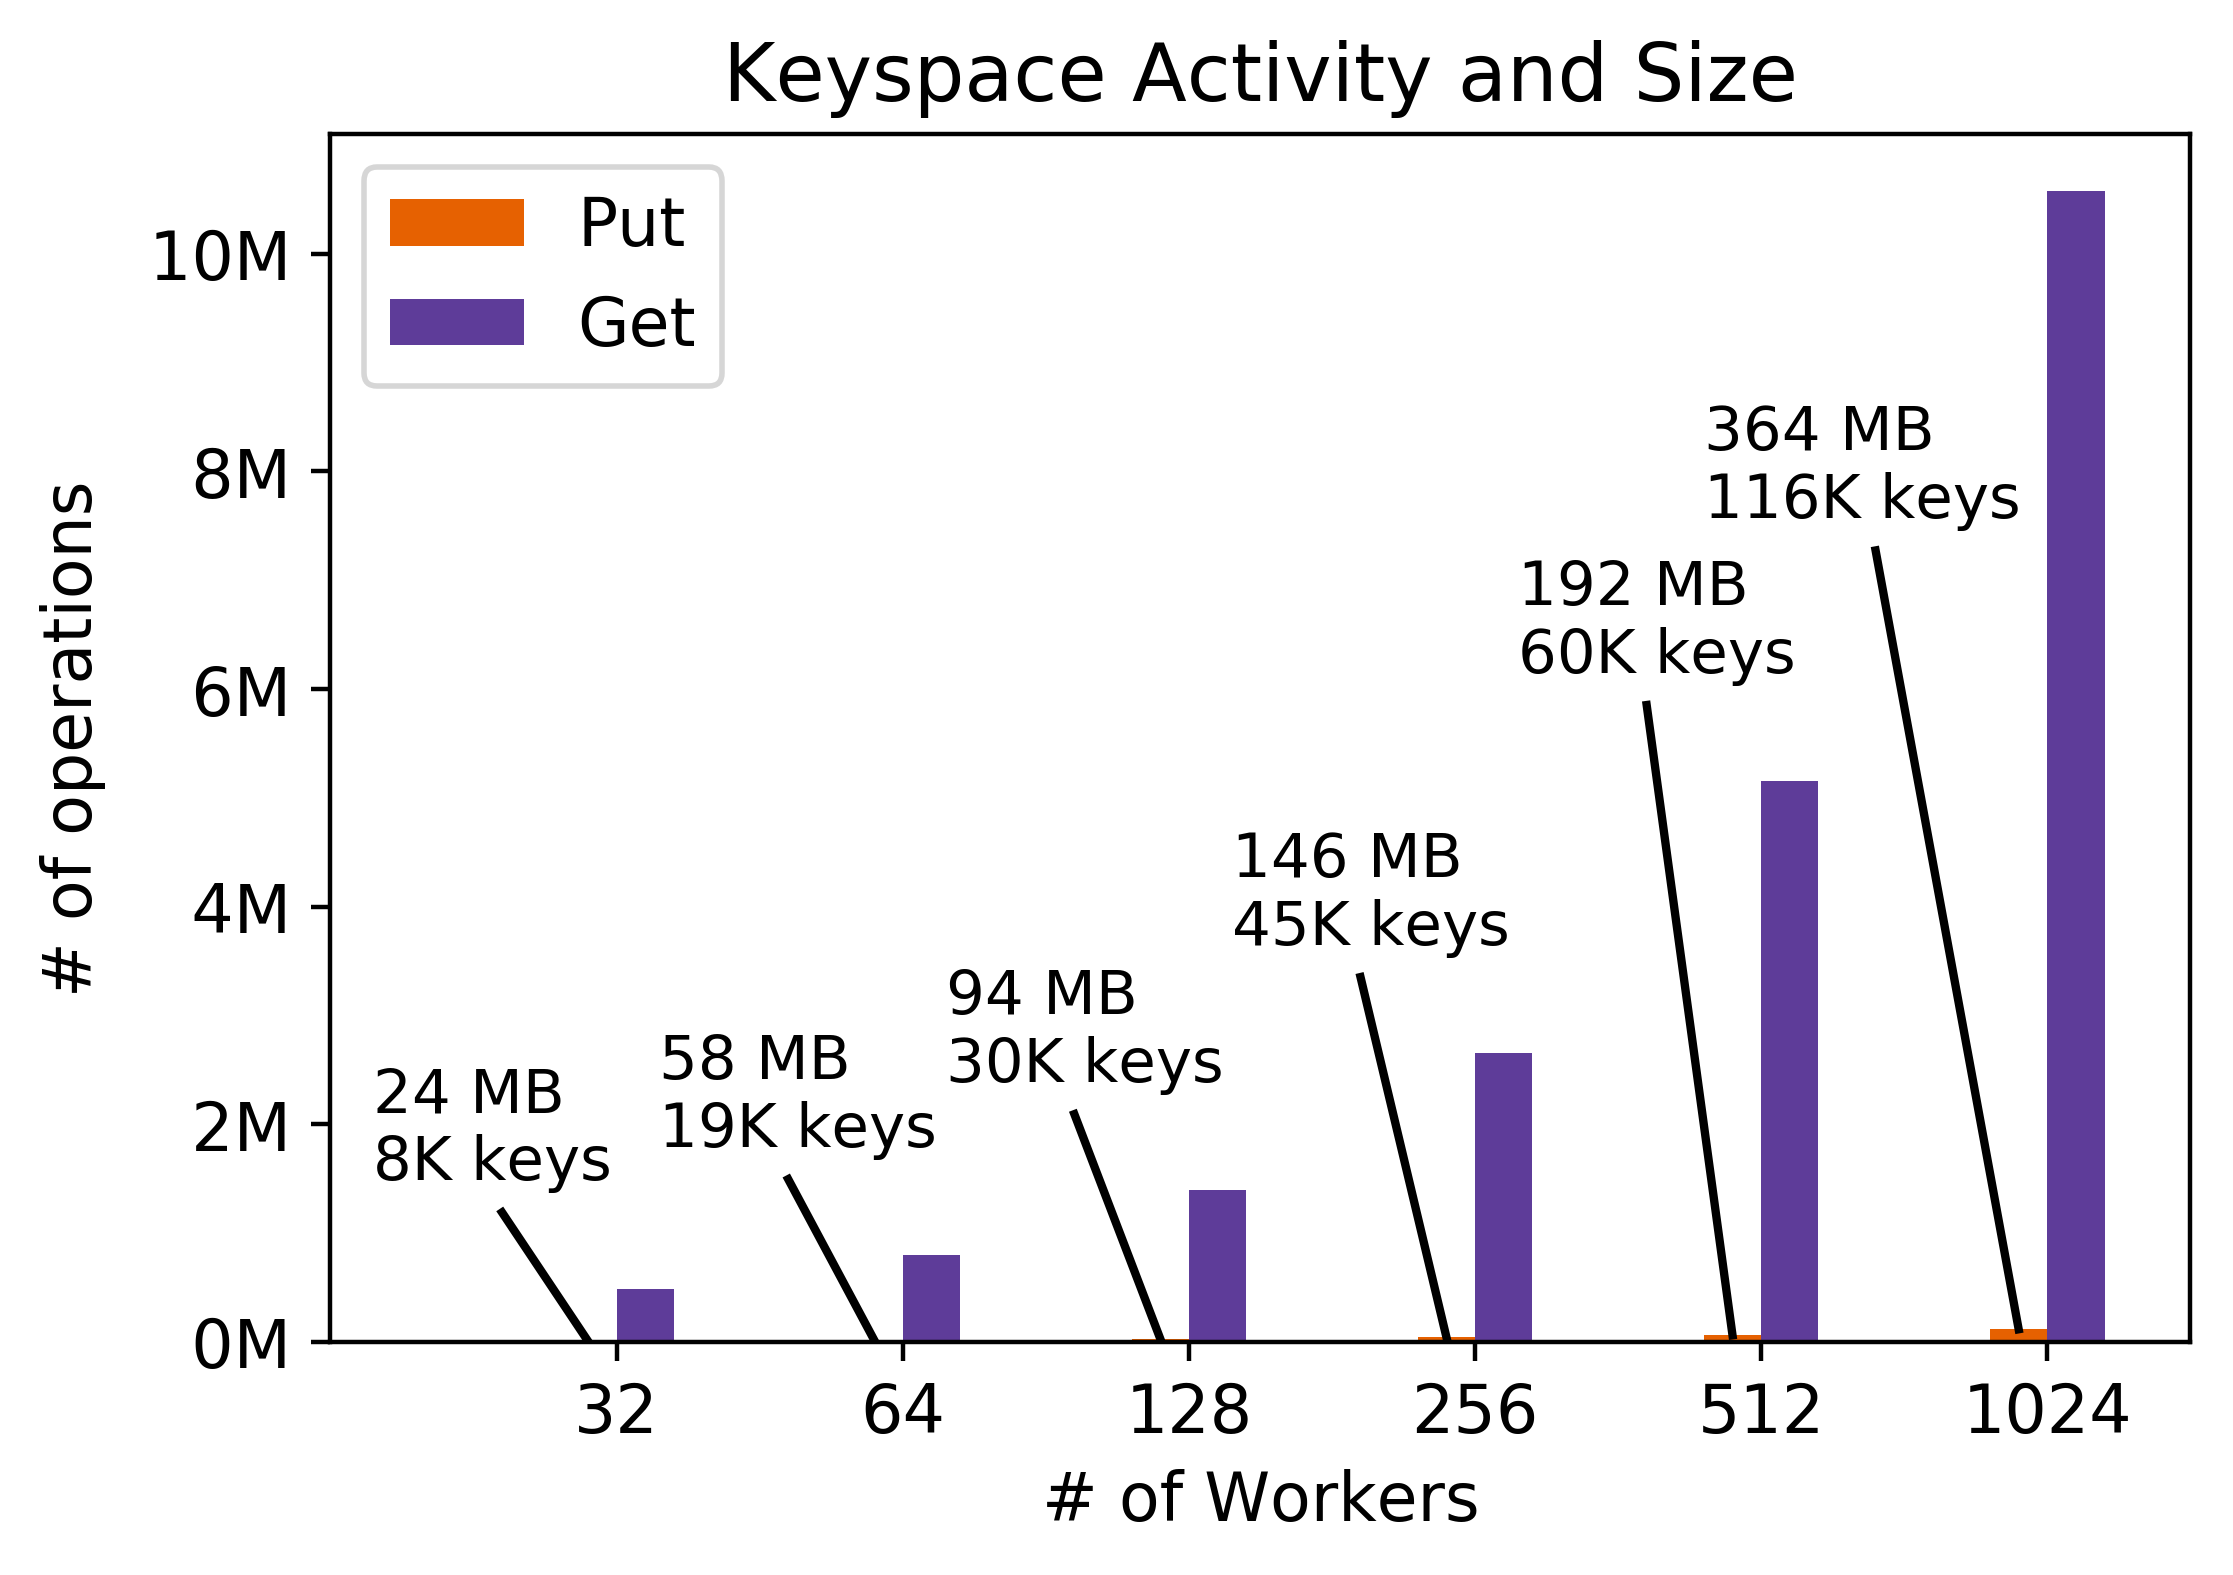
\includegraphics[width=0.4\textwidth]{figures/methodology-keyspace.png}\\
  \caption{The keyspace size is small but must satisfy many reads as workers
  calculate new segments. Based on these trends, it is likely that we will need
  more than one node to manage segment corodinates when we scale the system or jobs up.
  \label{fig:methodology-keyspace}}
\end{figure}

\begin{figure}[t]
  \noindent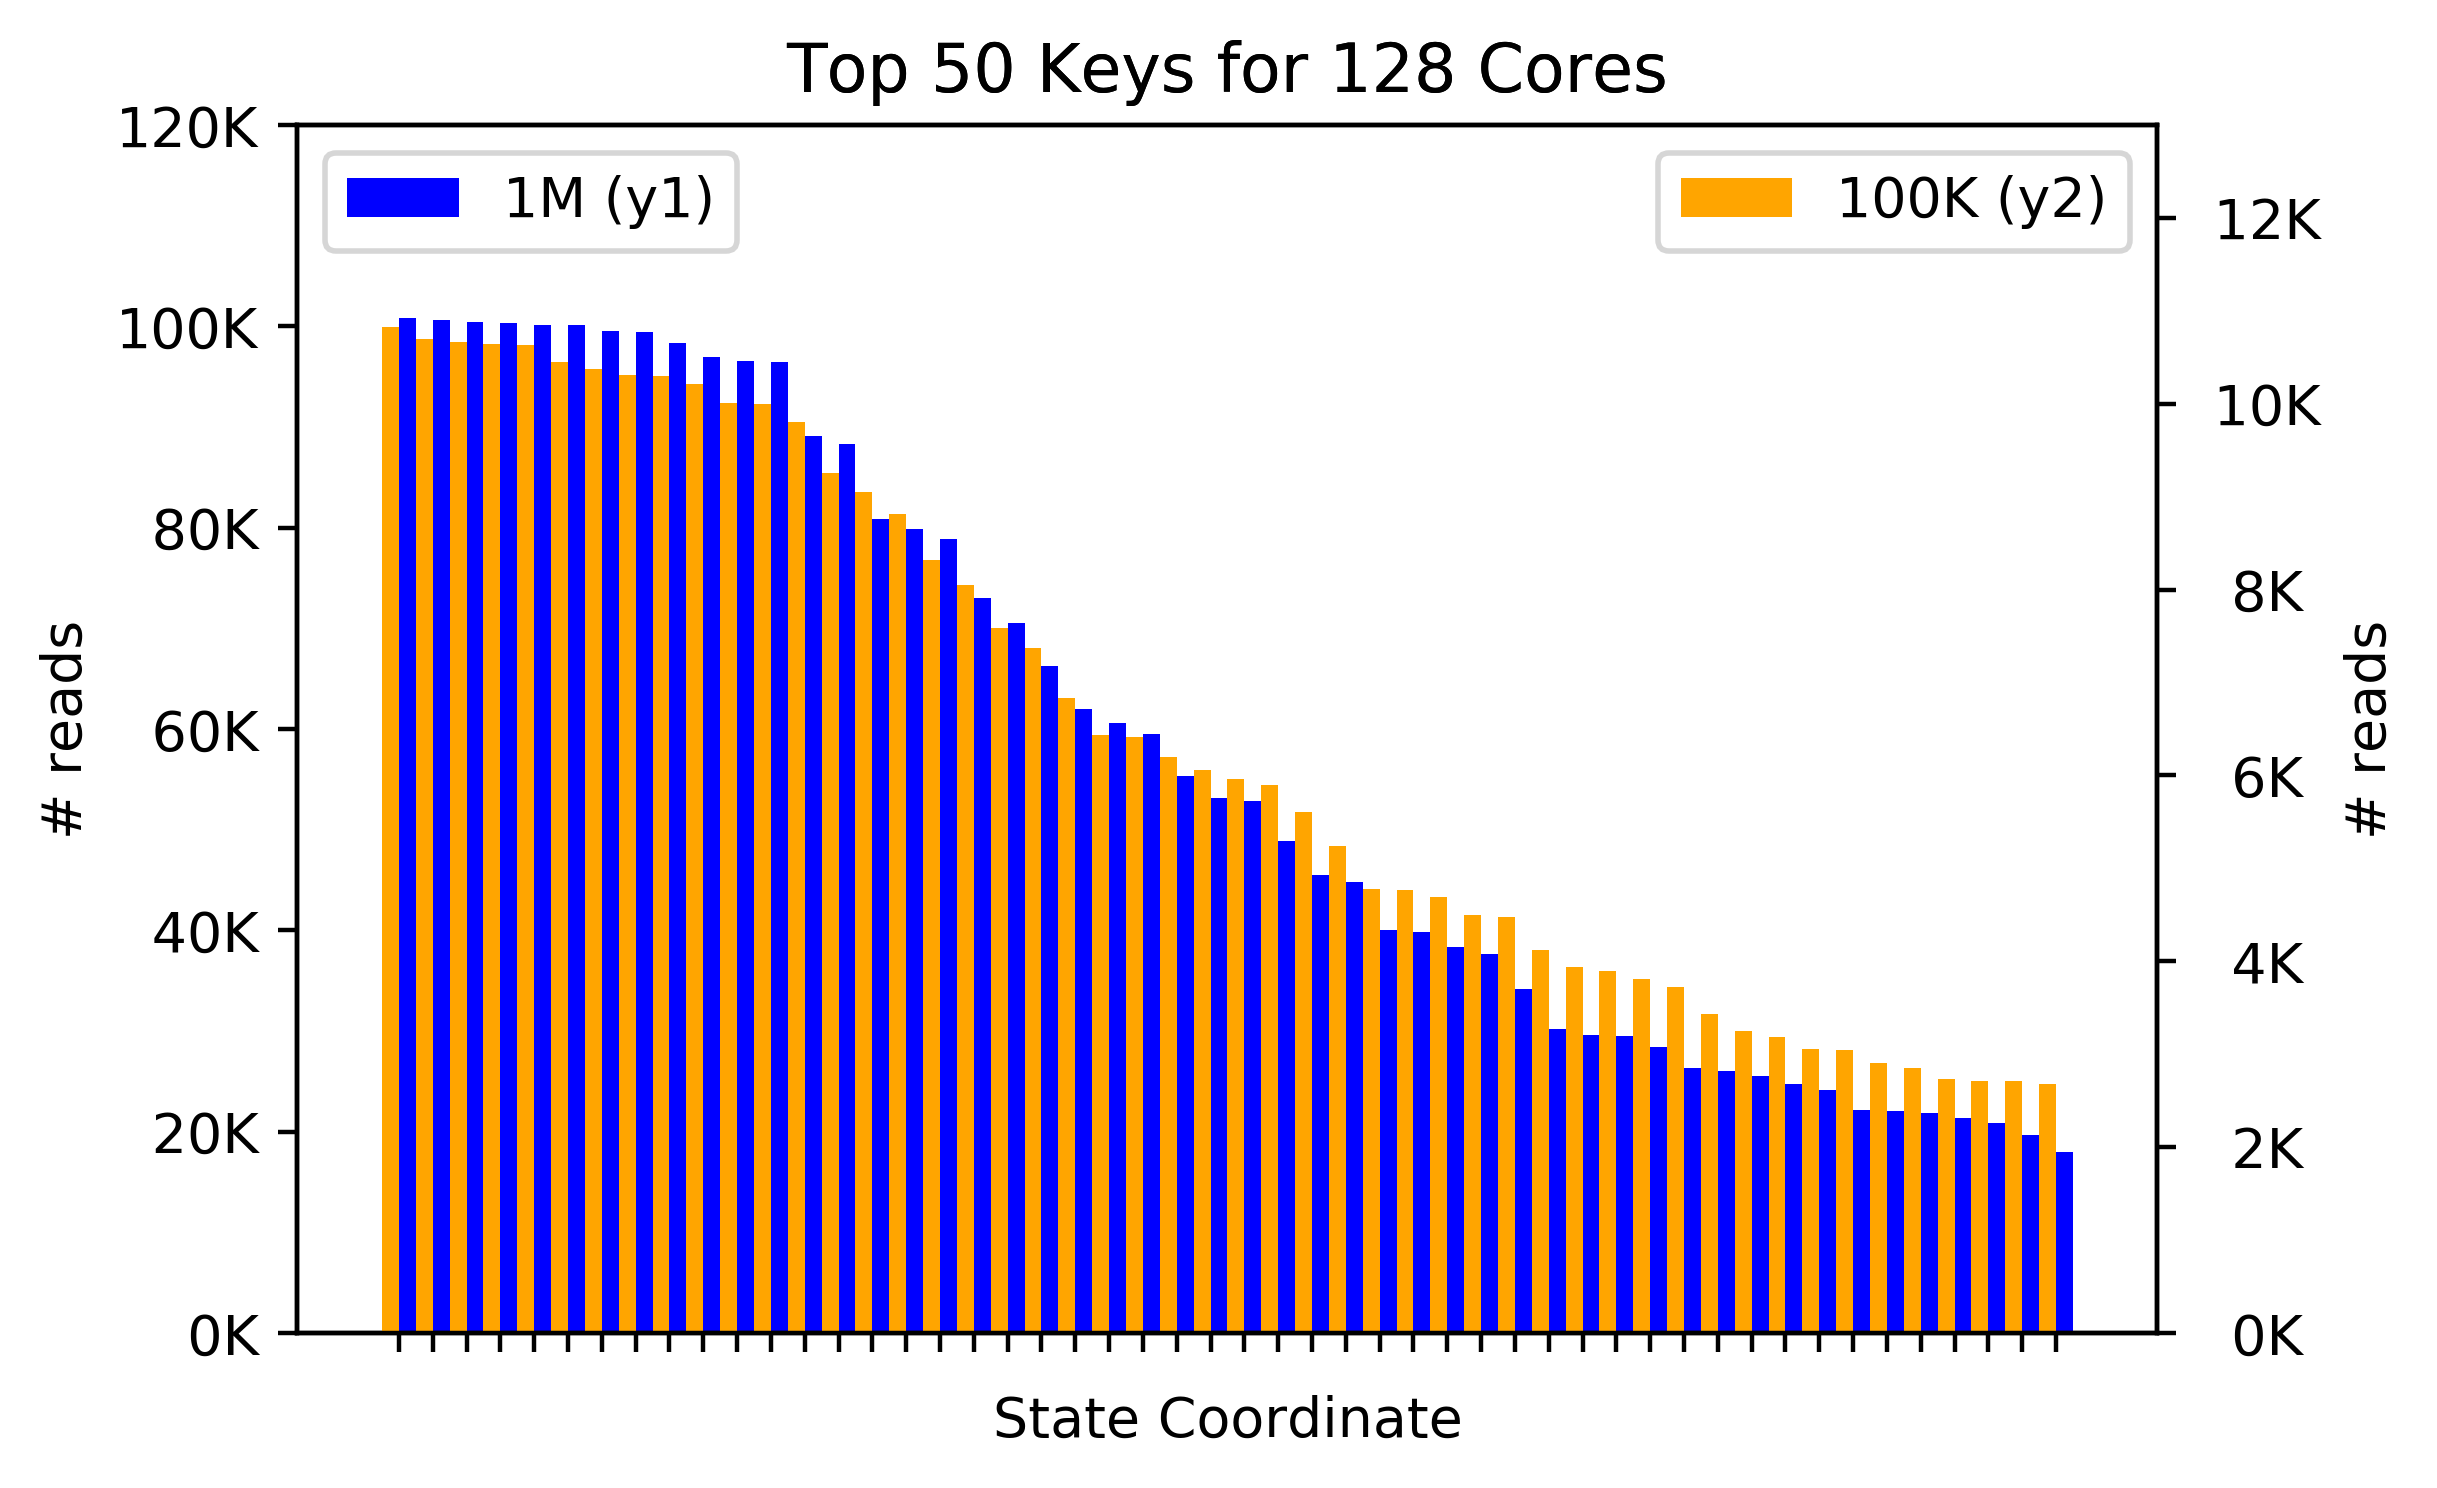
\includegraphics[width=0.4\textwidth]{figures/methodology-keys.png}\\
  \caption{The keyspace imbalance is due to workers generating deep
  trajectories and reading the same coordinates. Over time, the accesses get
  dispersed across different coordinates resulting in some keys being more
  popular than others.\label{fig:methodology-keys}}
\end{figure}

\subsubsection*{Scalability concerns} 
Figure~\ref{fig:methodology-keyspace} shows the keyspace size (black
annotations) and request load (bars) after a one hour run with a different
number of workers (\(x\) axis). While the keyspace size and capacity is
relatively modest the trends are concerning: memory usage scales with the
number of workers and Trinitite has 6000 cores. Furthermore, the size of the
keyspace scales with the length of the run. Extrapolating these magnitudes puts
an 8 hour run across all 100 Trinitite nodes at 20GB for the cache, which, in
addition to the 30GB base memory that ParSplice uses, puts the memory usage far
above the 4\% threshold we set earlier.

\subsubsection*{An active but small keyspace} 
The bars show \(50-100\times\) as many reads (\texttt{get()}) as writes
(\texttt{put()}).  Worker tasks read the same key for extended periods because
the trajectory segment is stuck in a superbasin composed of local minima, so
many coordinates are needed before the trajectory moves on. Writes only occur
for the final state of segments generated by worker tasks; their magnitude is
smaller than reads because the caches ignore redundant write requests. The
number of read and write requests are highest at the beginning of the run when
worker tasks generate segments for the same state, which is cheap. This type of
keyspace encourages replication across a cluster.  

\subsubsection*{Entropy increases over time} The reads per second in
Figure~\ref{fig:futurework-regimes} show that the number of requests decreases
and the number of active keys increases over time. The resulting key access
imbalance for the two growth rates in Figure~\ref{fig:futurework-regimes} are
shown in Figure~\ref{fig:methodology-keys}, where reads are plotted for each
unique state (\(x\) axis). Keys are more popular than others (up to
\(5\times\)) because worker tasks start generating states with different
coordinates later in the run.

\subsubsection*{Entropy growth is structured} The access patterns reflect the
locality of computation: worker tasks stuck in state basins generate segments with
similar coordinates. The growth rate, temperature, and number of workers
changes that locality, which has an effect on the structure of the keyspace.
Figure~\ref{fig:methodology-keys} shows that the number of reads changes with
different growth rates, but that spatial locality is similiar ({\it e.g.}, some
keys are stil \(5\times\) more popular than others).
Figure~\ref{fig:futurework-regimes} shows how entropy for different growth
rates has temporal locality, as the reads per second for 1M looks like the
reads per second for 100K stretched out along the time axis.  Trends also exist
for temperature and number of workers but are ommitted here for space. This
structure means that we can learn the regimes and adapt the storage system to
it. 
